\section{Exploring The Limits Of The Model}\label{seq:limits}
In this section we explore the limits of our model with regards to the input data.
%We first examine the scalability of the approach, then we evaluate the sensitivity of the approach to perturbation of the data.
All those experiments are performed on randomly generated data to have a control of the specific properties we want to evaluate.
%(in terms of performance)
    
\subsection{Problems With The Variational Part Of The Auto-Encoder}
When adding the KL loss to our prototype (initially a simple auto-encoder) the performance of the model was greatly impaired.
Analyzing the predictions revealed the model was going for ``low hanging fruits'' and ignored the embeddings themselves, as described in~\cite{annealing-kl:2015:bowman}.
To solve this problem we apply the annealing method of~\cite{annealing-kl:2015:bowman} and multiply the KL term by a lambda that we set to $0.2$.
This reduces the impact of the KL loss on the training and allows the model to learn some features before the KL loss comes into effect.
On the other hand, it reduces the benefits we get from using a VAE.%\todo{Replace with "It reduces the benefits we get from using a VAE though."}
    
\subsection{Reconstruction Performance}
In our initial experimentation we examine the reconstruction performance of the BoA auto-encoder.
We use the area under the receiver operating characteristics curve (AUC ROC) as a score.
It allows us to determine if the model has good predictive capacity without using an arbitrary threshold on the predicted value.
Additionally, AUC ROC gives a general account of performance, similarly to the F1 measure, as the receiver operating characteristics curve depends on precision and recall.
AUC ROC goes from 0 to 1, with results close to $0.5$ corresponding to poor predictive performance and those closer to $1$ correspond to better models.
To determine if the results are significantly different, we use Student t-test on means.
The results are presented in \autoref{fig:limits_concepts}.

\begin{figure}[t]
\begin{subfigure}{.48\textwidth}\centering
    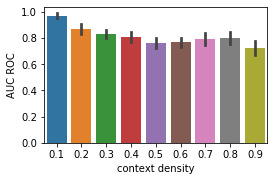
\includegraphics[width=\textwidth, height=3.8cm, keepaspectratio]{img/limits_densities.png}  
    \caption{Impact of the density, from 0.1 to 0.9, 100 samples per density.}\label{fig:limits_density}
\end{subfigure}\hspace{.03\textwidth}
\begin{subfigure}{.48\textwidth}\centering
    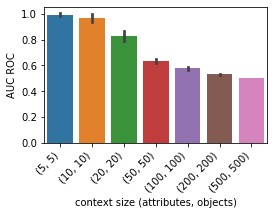
\includegraphics[width=\textwidth, height=3.8cm, keepaspectratio]{img/limits_size.png}  
    \caption{Impact of the size, from 5 to 500 objects and attributes, 20 samples per size.}\label{fig:limits_size}
\end{subfigure}\\
\begin{subfigure}{\textwidth}\centering
    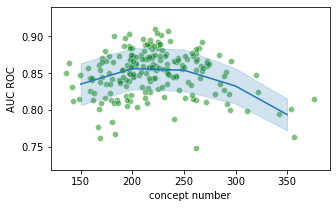
\includegraphics[height=5cm, keepaspectratio]{img/limits_concepts.png}  
    \caption{Impact of the concept number, for 200 sample with 20 objects and 20 attributes. The green dots are the actual results. The blue line is the general tendency when rounding the concept number to 50, the shaded area is the standard deviation.}\label{fig:limits_concepts}
\end{subfigure}
\caption{Reconstruction performance on random contexts. The error bars correspond to the standard deviation.}\label{fig:limits}
\end{figure}

% \begin{table}[t]
% \caption{Reconstruction performance on random contexts (mean $\pm$ std.).}\label{tab:limits}
% \centering
% \subfloat[Impact of the size ($|O| \times |A|$), 20 samples per size.]{\centering
% \begin{tabular}{lcl}
% \toprule
% context size &&   AUC ROC            \\
% \midrule
% $5 \times 5$       &&  $0.99\pm0.011$ \\
% $10 \times 10$     &&  $0.97\pm0.030$ \\
% $20 \times 20$     &&  $0.83\pm0.041$ \\
% $50 \times 50$     &&  $0.63\pm0.016$ \\
% $100 \times 100$   &&  $0.58\pm0.010$ \\
% $200 \times 200$   &&  $0.53\pm0.005$ \\
% $500 \times 500$   &&  $0.50\pm0.001$ \\
% \bottomrule
% \end{tabular}}
% \hfill
% \subfloat[Impact of the density, 100 samples per density.]{\centering
% \begin{tabular}{lcl}
% \toprule
% context density && AUC ROC             \\
% \midrule
% 0.1             &&  $0.97\pm0.02$ \\
% 0.2             &&  $0.87\pm0.04$ \\
% 0.3             &&  $0.83\pm0.03$ \\
% 0.4             &&  $0.81\pm0.04$ \\
% 0.5             &&  $0.76\pm0.04$ \\
% 0.6             &&  $0.77\pm0.03$ \\
% 0.7             &&  $0.79\pm0.04$ \\
% 0.8             &&  $0.80\pm0.05$ \\
% 0.9             &&  $0.72\pm0.05$ \\
% \bottomrule
% \end{tabular}}
% \end{table}

%\subsubsection{Impact Of The Density}
We first evaluate the impact of the density on the reconstruction AUC ROC.
We compare the performance on random contexts with densities from 0.1 to 0.9, with a fixed size of 20 objects and 20 attributes.
We use 100 samples per density.
Student's t-test show significant differences between the performance with the various densities: all the p-values are under 0.01 except between 0.4 and 0.8 (0.24), 0.5 and 0.6 (0.39), and 0.7 and 0.8 (0.19).
However, the model performance stays overall stable across the densities, while slightly better with smaller densities.
We suspect this tendency is due to the composition process of the object embeddings: the higher the density, the more attributes are present for an object, so more attribute embeddings are involved in the composition of the object embeddings, making it more complex to decode.

%\subsubsection{Impact Of The Size}
We also examine the effect of the size on the AUC ROC.
Square random contexts ($|O|=|A|$) of sizes in $\{5,10,20,50,100,200,500\}$ and a fixed density of 0.3 are used for this experiment.
We use 20 samples per size.
The model performs very well for seen data sizes with a slight drop to $0.83$ for $20$ objects and attributes.
When manipulating larger contexts the performance drops as we can expect.
For $50$ objects and attributes ($2.5$ times the maximum seen size), the AUC ROC is above $0.63$, but from $100$ objects and attributes onward, it drops under $0.6$.
Finally, with 500 objects and attributes (25 times the largest seen data size and 4 times the embedding size), the reconstruction AUC ROC falls to $0.50$ in average.
This is the limit of reconstruction performance with the current training process.

%\subsubsection{Impact Of The Concept Number}
\todo{Check this section with the FCA experts}
Finally, we examine the impact of the number of concepts on the performance of the model.
We use contexts of fixed size (20 objects and 20 attributes) from the test set, totaling 200 contexts.
We can\todo{Remove "can" ?} consider the concept number as an indicator of the variety of attributes and objects in the context.
Indeed, if the concept number is high for a given size of context, we can expect the context to be close to the clarified context. This implies a lower amount of duplicate objects and attributes.
In addition, we can expect the model to have a harder time encoding and decoding irregular contexts than repetitive ones.
Consequently, the drop of the AUC ROC for higher concept numbers is not surprising.
However, we also observe a lower performance around $150$ concepts.
Determining the cause of this second decrease requires further investigation.
%\todo{Find a plausible reason for the drop at $150$ concepts}
%Globally, the worst performance is still above 0.75, which is 

\subsection{Metric Learning Performance}
\begin{figure}[t]
\begin{subfigure}{.48\textwidth}\centering
    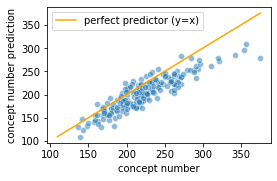
\includegraphics[height=4cm,width=\textwidth, keepaspectratio]{img/metric_concept_number.png}  
    \caption{Concept number.}\label{fig:metric_concept}
\end{subfigure}
\begin{subfigure}{.48\textwidth}\centering
    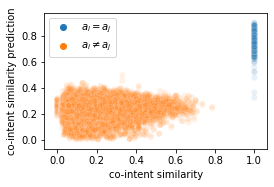
\includegraphics[height=4cm,width=\textwidth, keepaspectratio]{img/metric_cointent.png}  
    \caption{Co-intent similarity.}\label{fig:metric_cointent}
\end{subfigure}
\caption{Predicted pseudo-metrics against the actual values, for the 200 sample with 20 objects and 20 attributes from the test set.}\label{fig:metric}
\end{figure}

We evaluate the performance of the model for the co-intent similarity and number of concept prediction.
To obtain the predictions, we embed the attributes and apply the predictors trained togetner with the BoA model.
We use the 200 contexts of 20 objects and attributes from our test set.
The prediction results are reported \autoref{fig:metric}.

%Predicting the concept number value from an unordered composition of the attribute embeddings appears challenging.\todo{explain why challenging, and plpace it correctly in the paragraph}

The concept number prediction has a average error of $21.6$ and a standard deviation of $15.3$.
However, we can notice the tendency of the model to under-evaluate the concept number.
Also, the Pearson correlation coefficient is $0.9$ between the real value and the prediction, which indicates a strong correlation.
If we add $20$ to all the predictions, the average and standard deviation of the error fall to $14.6$ and $11.7$ respectively.
This corresponds to less than 10\% of error in the range of concepts of the seen data.
Overall, the prediction of the concept number is satisfying.
% and the p-value for testing non-correlation of $9.3 \times 10_{-74}$

For co-intent similarity however, the performance is not as encouraging.
The model manages to differentiate, for the similarity of $a_i$ and $a_j$, when $a_i = a_j$.
However, we do not find a salient tendency when $a_i \neq a_j$.
It seems that the model predictions for similarities between $0$ and $0.8$ are randomly picked between $0$ and $0.4$.
It appears the model has trouble learning the co-intent similarity.
Our investigation reveals a very small difference of the MSE between the first and last training epochs: from $0.17$ to $0.05$.
Using MSE on values between 0 and 1 seem to cause the problem: a MSE of $0.05$ corresponds to an actual distance of around $0.22$, so 10\% of the interval of definition.
We envision several solutions, like changing the loss to \textit{mean absolute error} (MAE) or normalizing the similarity.

%-> normalisation (log, exp,...) [0;1] ~> [0;inf[
%Suggestion mean-variance norm
